\chapter{Implementation}\label{implementation}

\section{Implementation Overview}\label{implementation-overview}

\begin{figure}[htbp]
\centering
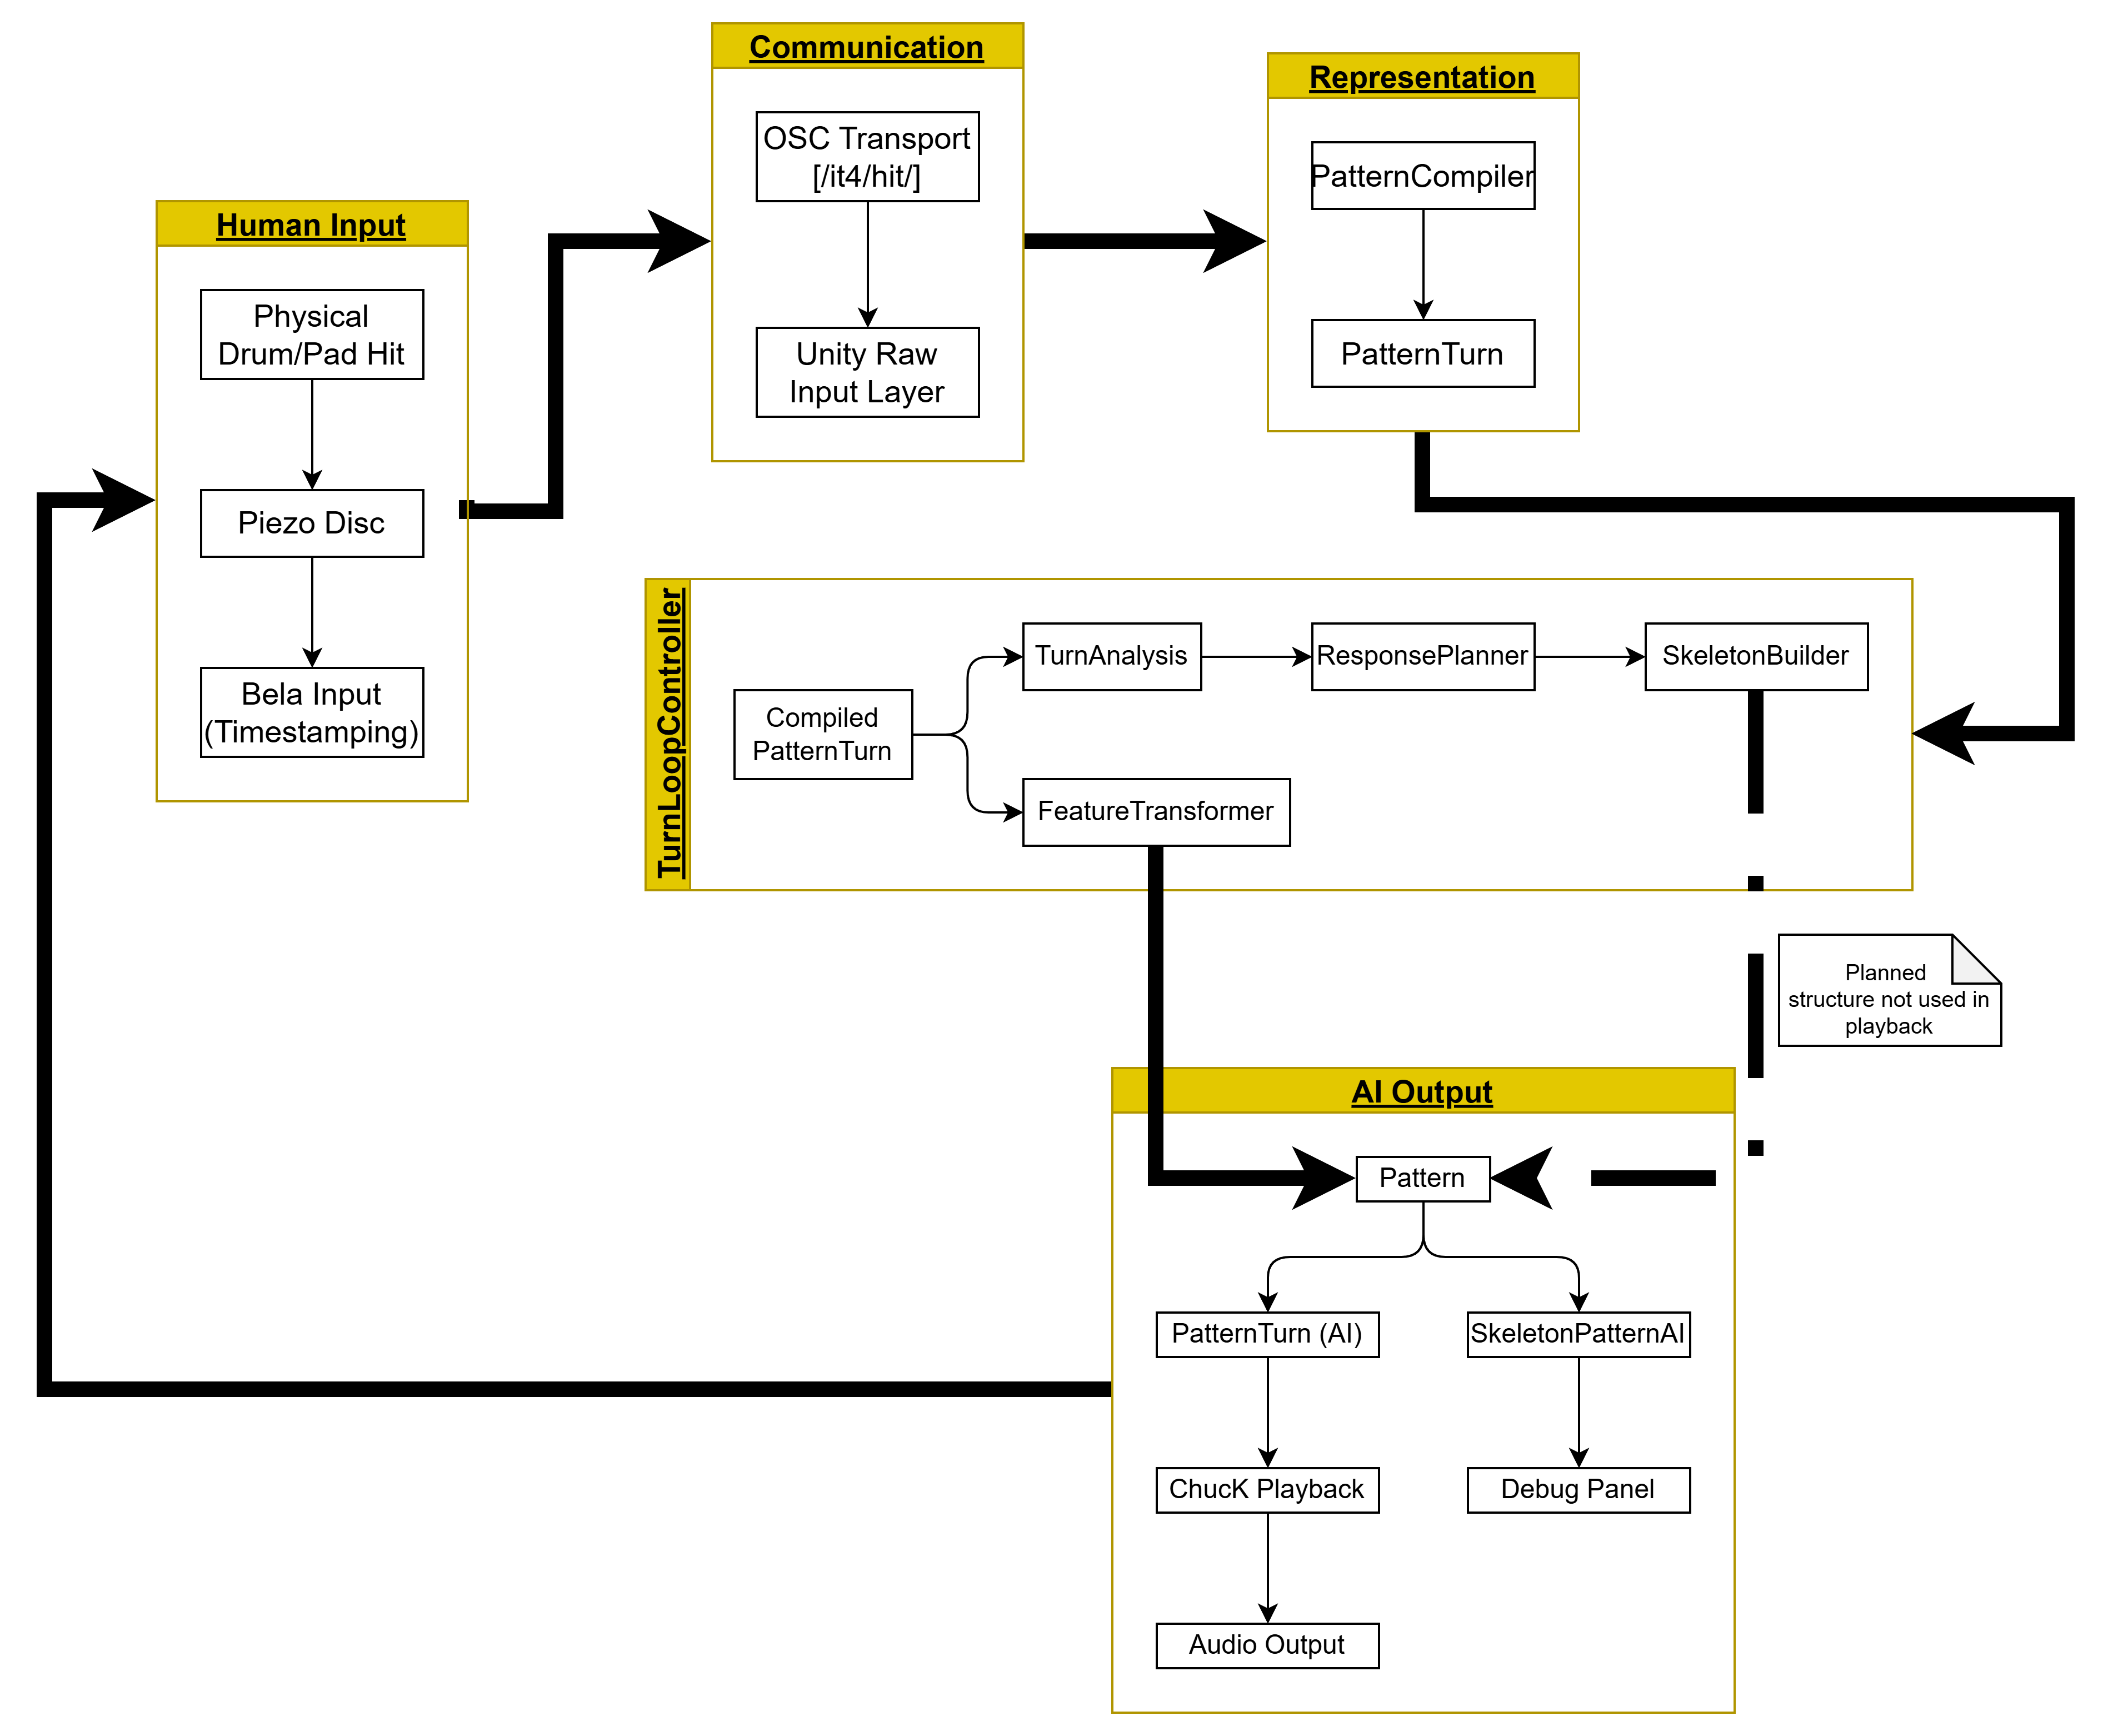
\includegraphics[width=\textwidth]{Figures/4 Figs/Global System Diagram.png}
\caption{High-level Intelli-Trading Fours system architecture.}
\label{fig:global-system-diagram}
\end{figure}

Figure~\ref{fig:global-system-diagram} presents a high-level overview of the Intelli-Trading Fours
system architecture, illustrating the complete pipeline from physical
drum interaction to audible AI response. The system is structured as a
sequence of transformation stages, in which rhythmic input is
progressively converted from continuous physical signals into symbolic
representations, analysed to extract musical features and transformed
into an output response.

\subsection{Modular structure}\label{modular-structure}

The architecture is organised into distinct functional modules, as shown
in Figure~\ref{fig:global-system-diagram}:

\begin{longtable}[]{@{}
  >{\raggedright\arraybackslash}p{(\linewidth - 4\tabcolsep) * \real{0.1743}}
  >{\raggedright\arraybackslash}p{(\linewidth - 4\tabcolsep) * \real{0.3471}}
  >{\raggedright\arraybackslash}p{(\linewidth - 4\tabcolsep) * \real{0.4786}}@{}}
\caption{System architecture modules}\label{tab:system-architecture-modules}\\
\toprule\noalign{}
\begin{minipage}[b]{\linewidth}\centering
\textbf{Layer}
\end{minipage} & \begin{minipage}[b]{\linewidth}\centering
\textbf{Components}
\end{minipage} & \begin{minipage}[b]{\linewidth}\centering
\textbf{Responsibility}
\end{minipage} \\
\begin{minipage}[b]{\linewidth}\raggedright
Human Input
\end{minipage} & \begin{minipage}[b]{\linewidth}\raggedright
Piezo, Bela
\end{minipage} & \begin{minipage}[b]{\linewidth}\raggedright
Signal acquisition and timestamping
\end{minipage} \\
\begin{minipage}[b]{\linewidth}\raggedright
Communication
\end{minipage} & \begin{minipage}[b]{\linewidth}\raggedright
OSC Transport, Unity Input Layer
\end{minipage} & \begin{minipage}[b]{\linewidth}\raggedright
Event transmission and reconstruction
\end{minipage} \\
\begin{minipage}[b]{\linewidth}\raggedright
Representation
\end{minipage} & \begin{minipage}[b]{\linewidth}\raggedright
PatternCompiler, PatternTurn
\end{minipage} & \begin{minipage}[b]{\linewidth}\raggedright
Quantisation and symbolic encoding
\end{minipage} \\
\begin{minipage}[b]{\linewidth}\raggedright
Orchestration
\end{minipage} & \begin{minipage}[b]{\linewidth}\raggedright
TurnLoopController
\end{minipage} & \begin{minipage}[b]{\linewidth}\raggedright
Turn segmentation and phase control
\end{minipage} \\
\begin{minipage}[b]{\linewidth}\raggedright
Reasoning
\end{minipage} & \begin{minipage}[b]{\linewidth}\raggedright
TurnAnalysis, ResponsePlanner
\end{minipage} & \begin{minipage}[b]{\linewidth}\raggedright
Feature extraction and decision-making
\end{minipage} \\
\begin{minipage}[b]{\linewidth}\raggedright
Structural
\end{minipage} & \begin{minipage}[b]{\linewidth}\raggedright
SkeletonBuilder
\end{minipage} & \begin{minipage}[b]{\linewidth}\raggedright
Structural response generation
\end{minipage} \\
\begin{minipage}[b]{\linewidth}\raggedright
Output
\end{minipage} & \begin{minipage}[b]{\linewidth}\raggedright
FeatureTransformer
\end{minipage} & \begin{minipage}[b]{\linewidth}\raggedright
Audible pattern generation
\end{minipage} \\
\begin{minipage}[b]{\linewidth}\raggedright
Playback
\end{minipage} & \begin{minipage}[b]{\linewidth}\raggedright
ChucK
\end{minipage} & \begin{minipage}[b]{\linewidth}\raggedright
Real-time audio rendering
\end{minipage} \\
\midrule\noalign{}
\endhead
\bottomrule\noalign{}
\endlastfoot
\end{longtable}


\section{Bela Hardware Input \& OSC Transport}\label{bela-hardware-input-osc-transport}

The system captures physical drum interactions using a piezoelectric
sensor connected to a Bela embedded audio platform. This stage converts
mechanical impact into timestamped digital events which are transmitted
to the Unity environment via OSC.

\subsection{Hardware Configuration}\label{hardware-configuration}

\begin{figure}[htbp]
\centering
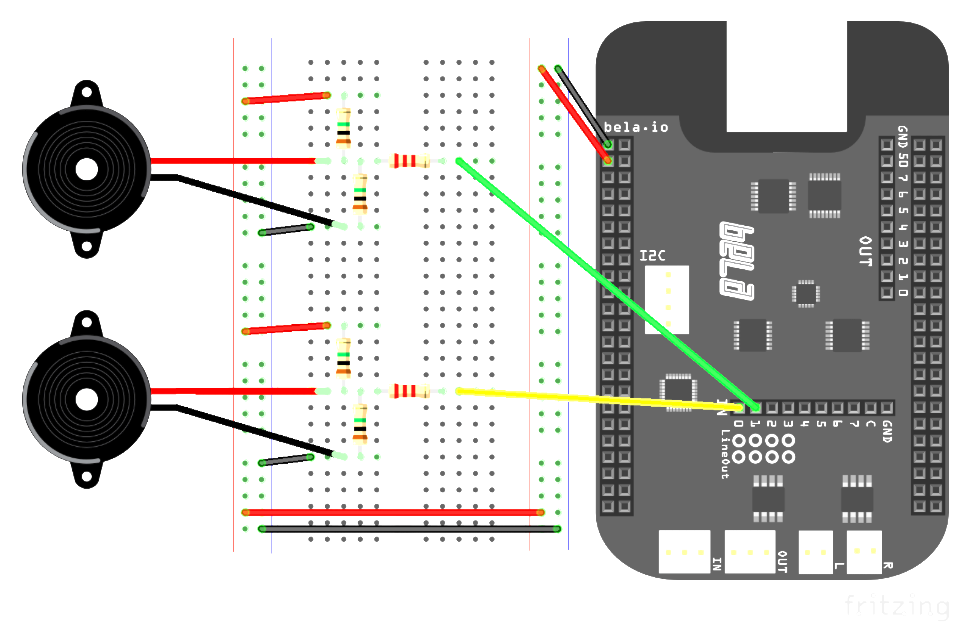
\includegraphics[width=\textwidth]{Figures/Piezo x Bread Board.png}
\caption{Piezo sensor and breadboard hardware input arrangement.}
\label{fig:piezo-breadboard}
\end{figure}

\begin{figure}[htbp]
\centering
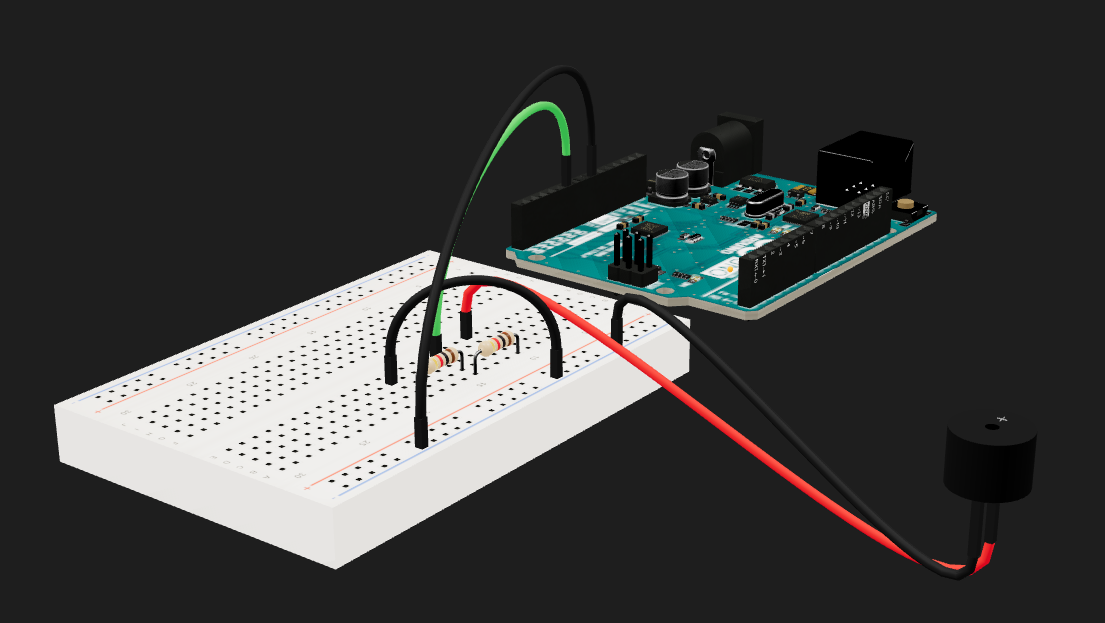
\includegraphics[width=\textwidth]{Figures/4 Figs/Simulated Hardware (Side View 1).png}
\caption{Simulated hardware side view showing the signal path from sensor to Bela input.}
\label{fig:hardware-side-view-1}
\end{figure}

\begin{figure}[htbp]
\centering
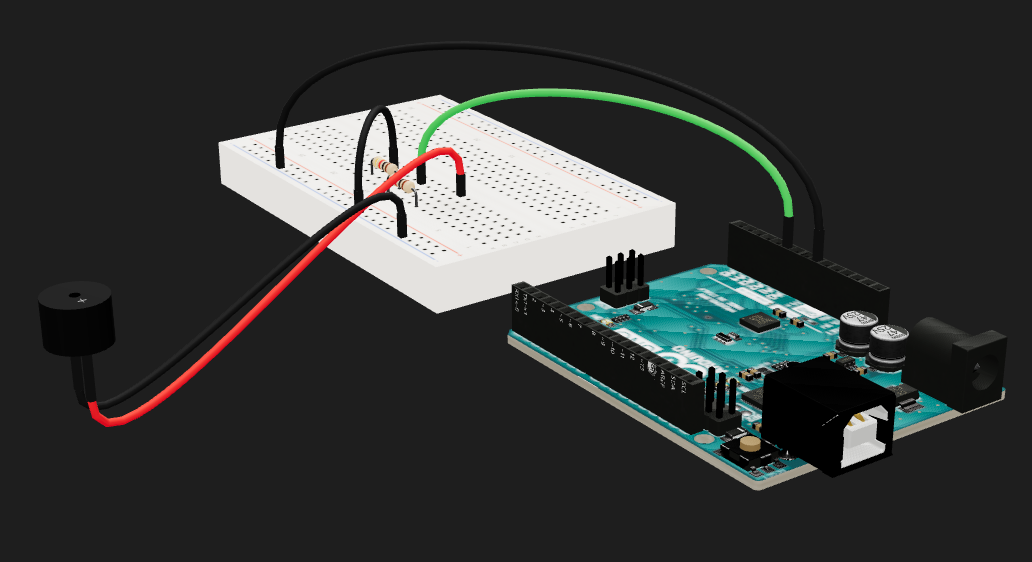
\includegraphics[width=\textwidth]{Figures/4 Figs/Simulated Hardware (Side View 2).png}
\caption{Alternate simulated hardware side view showing component placement.}
\label{fig:hardware-side-view-2}
\end{figure}

\begin{figure}[htbp]
\centering
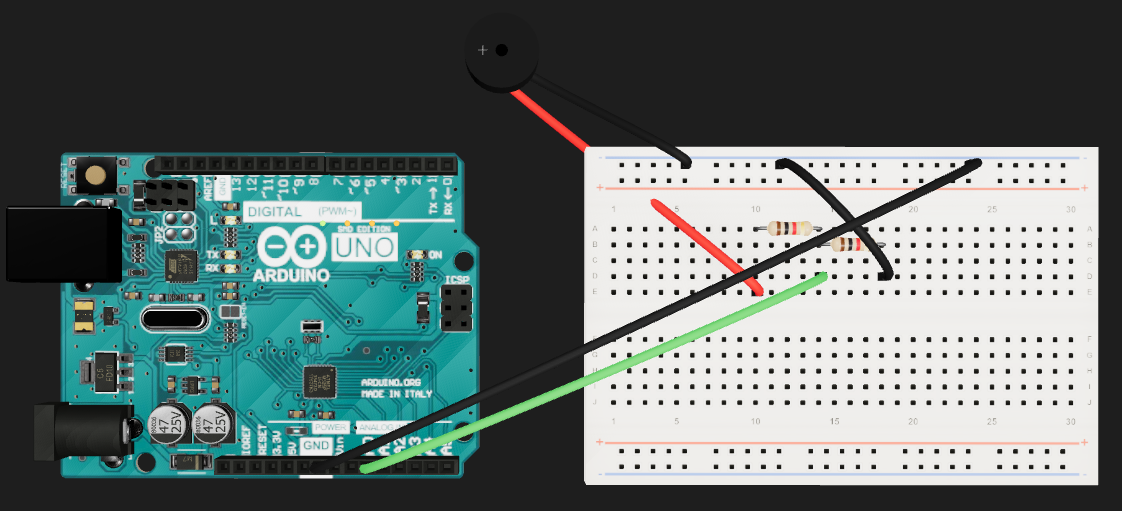
\includegraphics[width=\textwidth]{Figures/4 Figs/Simulated Hardware (Top View).png}
\caption{Simulated hardware top view showing breadboard layout and routing.}
\label{fig:hardware-top-view}
\end{figure}

The hardware configuration consists of a single piezo disc connected to
a breadboard-based resistor network, interfacing directly with a Bela
analog input channel. The accompanying figures illustrate the physical
implementation from multiple perspectives.

The side-view figures highlight the linear signal path from the piezo
sensor to the Bela input, while the top-view figure clarifies the
breadboard layout, grounding and resistor placement. Together, these
views make explicit both the electrical connectivity and the physical
routing of the signal.

The piezo sensor generates a transient voltage spike when struck, which
is routed through a passive conditioning circuit (series + bleed
resistor) before reaching the Bela input.

\subsection{Signal Path}\label{signal-path}

The input signal follows a linear path from mechanical interaction to
digital representation:

\begin{lstlisting}
Drum Hit -> Piezo Disc -> Voltage Spike -> Series Resistor -> Bela Analog Input
\end{lstlisting}

\begin{itemize}
\item
  The piezo disc converts mechanical deformation into voltage
\item
  The series resistor limits current and stabilises the input signal
\item
  The analog input on Bela samples the signal at audio rate
\end{itemize}

\subsection{Hit Detection}\label{hit-detection}

Hit detection is performed on the Bela side within the render.cpp
process which applies threshold-based logic to the incoming signal
stream.

For each sample:

\begin{lstlisting}
if signal(t) > threshold and refractory == false:
    register hit
\end{lstlisting}

\begin{itemize}
\item
  Thresholding filters noise and low-amplitude vibrations
\item
  Refractory period prevents multiple triggers from a single strike
\item
  Detection operates directly on the sampled signal
\end{itemize}

\subsection{Timestamping}\label{timestamping}

Each detected hit is assigned a timestamp using Bela's audio sample
clock:

\begin{itemize}
\item
  Sample rate: 44.1 kHz
\item
  Temporal resolution: \textasciitilde22.7 \(\mu\)s per sample
\end{itemize}

This provides high-precision timing for downstream quantisation.

\subsection{OSC Transmission}\label{osc-transmission}

Detected hits are transmitted to Unity via OSC on the /it4/hit address.

Message payload:

\begin{lstlisting}
(t_hi, t_lo, pad, velocity)
\end{lstlisting}

Where:

\begin{itemize}
\item
  t\_hi, t\_lo: a 64-bit sample timestamp reconstructed from two 32-bit
  integers
\item
  Pad: the input identifier (single pad in current system)
\item
  velocity: the amplitude-derived intensity
\end{itemize}

\subsection{System Integration}\label{system-integration}

The complete input pipeline:

\begin{lstlisting}
Piezo Signal
  -> Bela Sampling
  -> Hit Detection
  -> Timestamp Assignment
  -> OSC Transmission
  -> Unity HitEvent
\end{lstlisting}

\subsection{Role in System Architecture}\label{role-in-system-architecture}

This stage defines the transition from physical interaction to
computational input, producing timestamped hit events that form the
basis for all subsequent processing stages.

\section{Turn Orchestration and Temporal Segmentation}\label{turn-orchestration-and-temporal-segmentation}

The system transforms a continuous stream of timestamped hit events into
interaction units through a turn-based orchestration model, defining
when input is captured, how long it is processed and how interaction
alternates between human and system.

\subsection{Turn-Based Interaction Model}\label{turn-based-interaction-model}

\begin{figure}[htbp]
\centering
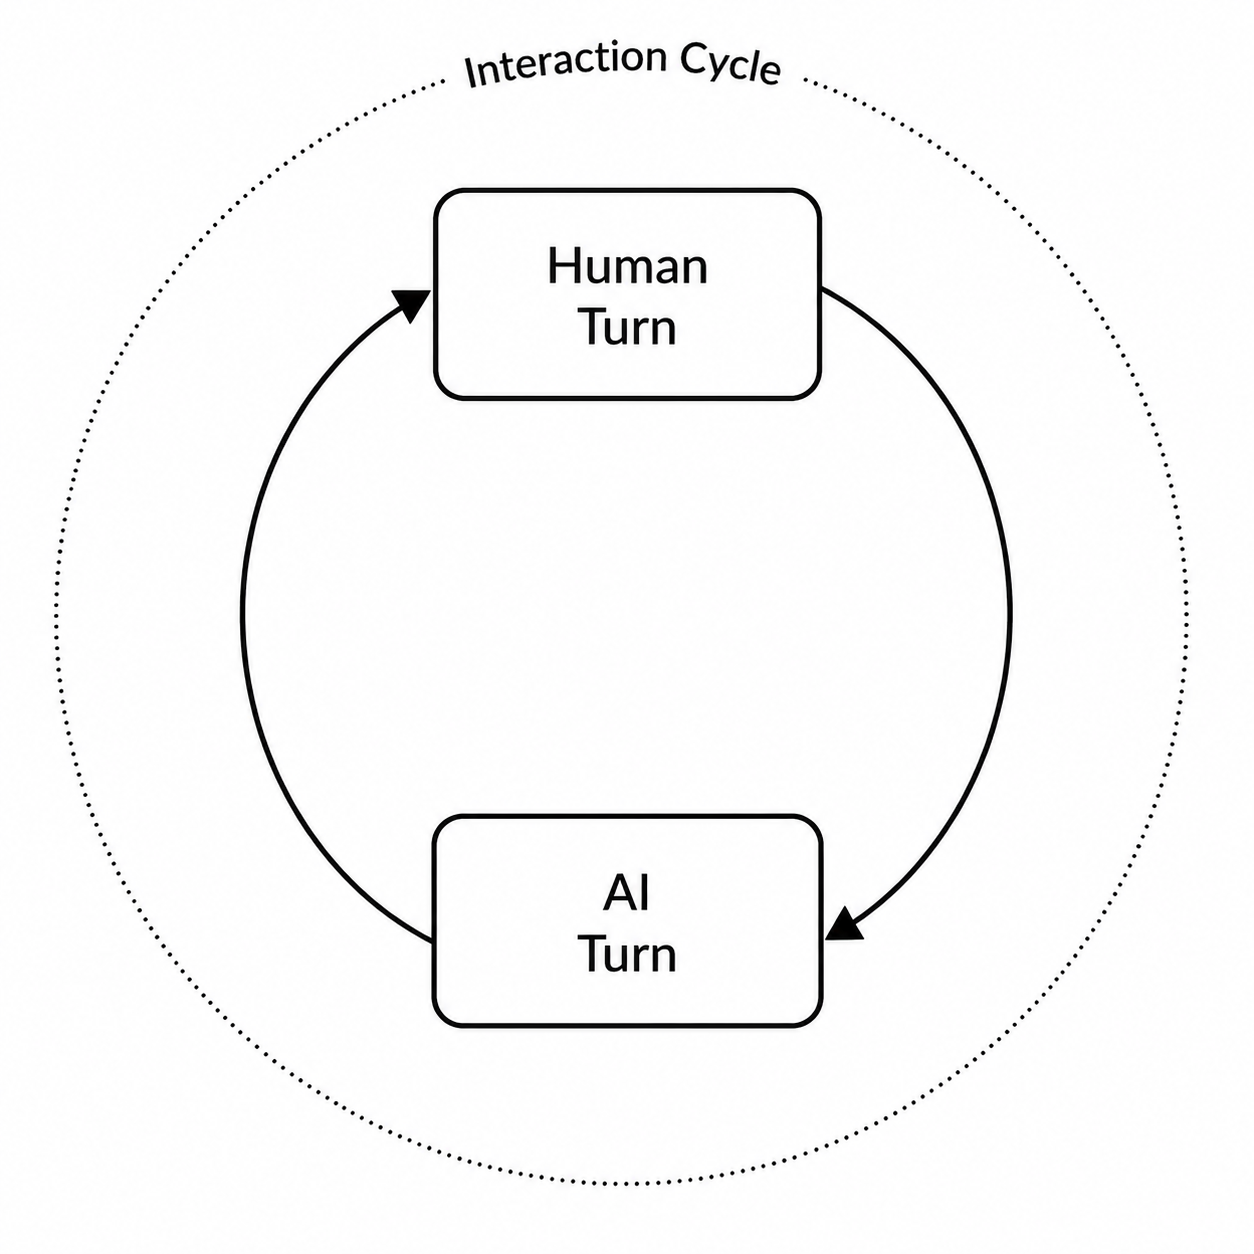
\includegraphics[width=\textwidth]{Figures/4 Figs/Interaction Cycle.png}
\caption{Turn-based interaction cycle used by the runtime orchestration model.}
\label{fig:interaction-cycle}
\end{figure}

Figure~\ref{fig:interaction-cycle} illustrates the interaction model as alternating turns. Each
turn is treated as a fixed-duration segment of rhythmic input or output.

\subsection{Turn Initiation}\label{turn-initiation}

A human turn is initiated by the first valid hit received during the
idle state. The timestamp of this hit defines the start of the turn
enabling event-driven segmentation rather than fixed-time slicing.

\subsection{Turn Duration}\label{turn-duration}

Turn length is fixed and derived from a preset tempo configuration:

\[
\mathrm{turnDuration} = \mathrm{bars} \times \mathrm{beatsPerBar} \times (60 / \mathrm{BPM})
\]

This ensures consistent structural length, compatible with the
quantisation grid and aligned with playback timing.

\subsection{Capture Window}\label{capture-window}

During a human turn:

\begin{itemize}
\item
  all incoming HitEvents are appended to the HitBuffer
\item
  events are stored with sample timestamps
\end{itemize}

The result is a TurnWindow object comprised of:

slice(HitBuffer, start, end)

\subsection{TurnWindow Structure}\label{turnwindow-structure}

This object contains:

\begin{itemize}
\item
  list of HitEvents
\item
  start timestamp
\item
  end timestamp
\end{itemize}

\subsection{Phase Control}\label{phase-control}

Turn progression is managed by TurnLoopController through phases that
indicate the current system state:

\begin{longtable}[]{@{}
  >{\raggedright\arraybackslash}p{(\linewidth - 2\tabcolsep) * \real{0.2171}}
  >{\raggedright\arraybackslash}p{(\linewidth - 2\tabcolsep) * \real{0.2813}}@{}}
\caption{TurnLoopController phases}\label{tab:turn-loop-phases}\\
\toprule\noalign{}
\begin{minipage}[b]{\linewidth}\centering
\textbf{Phase}
\end{minipage} & \begin{minipage}[b]{\linewidth}\centering
\textbf{Behaviour}
\end{minipage} \\
\begin{minipage}[b]{\linewidth}\raggedright
WaitingForHuman
\end{minipage} & \begin{minipage}[b]{\linewidth}\raggedright
idle, listening for first hit
\end{minipage} \\
\begin{minipage}[b]{\linewidth}\raggedright
CapturingHuman
\end{minipage} & \begin{minipage}[b]{\linewidth}\raggedright
recording input
\end{minipage} \\
\begin{minipage}[b]{\linewidth}\raggedright
Processing
\end{minipage} & \begin{minipage}[b]{\linewidth}\raggedright
analysis + planning
\end{minipage} \\
\begin{minipage}[b]{\linewidth}\raggedright
PlayingAI
\end{minipage} & \begin{minipage}[b]{\linewidth}\raggedright
output playback
\end{minipage} \\
\begin{minipage}[b]{\linewidth}\raggedright
Transition
\end{minipage} & \begin{minipage}[b]{\linewidth}\raggedright
reset + prepare next turn
\end{minipage} \\
\midrule\noalign{}
\endhead
\bottomrule\noalign{}
\endlastfoot
\end{longtable}


\subsection{Role in System Architecture}\label{role-in-system-architecture-1}

This stage defines the transition from continuous interaction to
discrete computational units, producing bounded segments ready for
deterministic processing by downstream modules.

\section{Symbolic Representation and Quantisation}\label{symbolic-representation-and-quantisation}

PatternTurn is the fixed symbolic representation of captured turn data.

\subsection{PatternTurn Structure}\label{patternturn-structure}

PatternTurn represents rhythm as a discrete time grid storing:

\begin{itemize}
\item
  Velocity{[}i{]}

  \begin{itemize}
  \item
    Hit intensity at step i (0-127)
  \end{itemize}
\item
  offsetSamples{[}i{]}

  \begin{itemize}
  \item
    Microtiming deviation from grid
  \end{itemize}
\item
  Metadata:

  \begin{itemize}
  \item
    BPM
  \item
    sampleRate
  \item
    stepsPerQuarter
  \end{itemize}
\end{itemize}

\subsection{Quantisation Process}\label{quantisation-process}

Each hit is snapped to a discrete grid position:

\[
\mathrm{stepIndex} = \mathrm{round}(\mathrm{sampleOffset} / \mathrm{samplesPerStep})
\]

Where:

\[
\mathrm{samplesPerStep} = (60 / \mathrm{BPM} / \mathrm{stepsPerQuarter}) \times \mathrm{sampleRate}
\]

\subsection{Collision handling}\label{collision-handling}

If multiple hits map to the same step:

\[
\mathrm{velocity}[\mathrm{step}] = \max(\mathrm{existing}, \mathrm{new})
\]

\subsection{Microtiming preservation}\label{microtiming-preservation}

Deviation from the grid is stored:

\[
\mathrm{offsetSamples}[\mathrm{step}] = \mathrm{actualTime} - \mathrm{quantisedTime}
\]

\subsection{Role in System Architecture}\label{role-in-system-architecture-2}

Representation and Quantisation define the transition from continuous
time signals to discrete symbolic structure, providing the input format
required for the reasoning and generation processes.

\section{Analysis, Planning \& Structural Generation}\label{analysis-planning-structural-generation}

\subsection{Runtime flow and module boundaries}\label{runtime-flow-and-module-boundaries}

% TODO: Missing UML diagram asset for PatternTurn to SkeletonPattern journey.

\subsection{TurnAnalysis: Modular Feature Extraction}\label{turnanalysis-modular-feature-extraction}

The Analysis stage is implemented as a modular feature extraction layer
where rhythmic descriptors are derived by a set of specialised analyser
components governed by a central Analysis orchestration class.

Rather than performing a single holistic analysis, the system decomposes
this process into a set of feature-specific computations, each capturing
a different aspect of rhythmic behaviour. These features are computed
directly from the quantised step grid and associated velocity values
(PatternTurn) - allowing the system to reason over both event
distribution and intensity.

\subsubsection{TurnAnalysis Structure}\label{turnanalysis-structure}

\begin{longtable}[]{@{}
  >{\raggedright\arraybackslash}p{(\linewidth - 2\tabcolsep) * \real{0.1620}}
  >{\raggedright\arraybackslash}p{(\linewidth - 2\tabcolsep) * \real{0.6289}}@{}}
\caption{TurnAnalysis module structure}\label{tab:turnanalysis-structure}\\
\toprule\noalign{}
\begin{minipage}[b]{\linewidth}\centering
\textbf{Layer}
\end{minipage} & \begin{minipage}[b]{\linewidth}\centering
\textbf{Responsibility}
\end{minipage} \\
\begin{minipage}[b]{\linewidth}\raggedright
Analysers
\end{minipage} & \begin{minipage}[b]{\linewidth}\raggedright
Feature-specific computation components
\end{minipage} \\
\begin{minipage}[b]{\linewidth}\raggedright
Models
\end{minipage} & \begin{minipage}[b]{\linewidth}\raggedright
Data structures for feature storage and aggregation
\end{minipage} \\
\begin{minipage}[b]{\linewidth}\raggedright
Utils
\end{minipage} & \begin{minipage}[b]{\linewidth}\raggedright
Shared utilities (e.g. segmentation, thresholds)
\end{minipage} \\
\begin{minipage}[b]{\linewidth}\raggedright
TurnAnalyser
\end{minipage} & \begin{minipage}[b]{\linewidth}\raggedright
Orchestrator governing execution and result aggregation
\end{minipage} \\
\midrule\noalign{}
\endhead
\bottomrule\noalign{}
\endlastfoot
\end{longtable}


The analysis module is organised into three functional layers,
supporting separation of concerns architecture

This structure allows feature computation to remain independent and
composable, enabling the analysis stage to be extended with additional
descriptors without modifying existing components.

At runtime, the orchestrator TurnAnalyser coordinates the execution of
the analyser components, aggregating their outputs into a single
TurnAnalysisResult object.

\subsubsection{Execution Pipeline}\label{execution-pipeline}

TurnAnalyser

\textbar{}

+-\/- DensityAnalyser

+-\/- EnergyAnalyser

+-\/- AnchorAnalyser

+-\/- EndActivityAnalyser

+-\/- SegmentActivityProfileAnalyser

\(\downarrow\)

TurnAnalysisResult

PatternTurn

\(\downarrow\)

DensityAnalyser

EnergyAnalyser

AnchorAnalyser

EndActivityAnalyser

\(\downarrow\)

SegmentActivityProfileAnalyser

\(\downarrow\)

TurnAnalysisResult

% TODO: Replace this placeholder with a UML diagram if the asset becomes available.

% TODO: Add explanatory text for the analysis pipeline figure once the diagram is finalised.

Execution is triggered during AI response preparation and occurs once
per captured human turn.

\subsubsection{Feature Computation}\label{feature-computation}

Each analyser applies a rule-based transformation to the input pattern,
producing a compact set of statistics or classifications that describe
the input at different levels of abstraction. Lower-level features, such
as density and energy, summarise global properties of the pattern, while
higher-level features, such as anchors and segment activity profiles,
capture structural and perceptual aspects of the rhythm.

\begin{longtable}[]{@{}llll@{}}
\caption{Analysis feature computation methods}\label{tab:analysis-feature-computation}\\
\toprule\noalign{}
\textbf{Analyser} & \textbf{Input} & \textbf{Output} &
\textbf{Method} \\
Density & step occupancy (velocity \textgreater{} 0) & step density,
active count, segment densities & count-based \\
Energy & active-step velocities & mean, peak, variance, segment means &
statistical \\
Anchors & velocity + step position & salience scores, anchor indices &
weighted scoring \\
End Activity & final quarter of turn & end density, energy, accent &
windowed summary \\
Segment Profile & segment features & activity shape classification &
pattern classification \\
\midrule\noalign{}
\endhead
\bottomrule\noalign{}
\endlastfoot
\end{longtable}


Table~\ref{tab:analysis-feature-computation} summarises the analyser inputs, outputs and methods.

\subsubsection{Anchor Detection}\label{anchor-detection}

Anchor detection assigns a salience score to each step in the pattern,
steps are classified as anchors when salience exceeds a threshold.

\paragraph{Computation}\label{computation}

For each step i where velocity{[}i{]} \textgreater{} 0:

\begin{longtable}[]{@{}
  >{\raggedright\arraybackslash}p{(\linewidth - 2\tabcolsep) * \real{0.2487}}
  >{\raggedright\arraybackslash}p{(\linewidth - 2\tabcolsep) * \real{0.4492}}@{}}
\caption{Anchor salience score components}\label{tab:anchor-score-components}\\
\toprule\noalign{}
\begin{minipage}[b]{\linewidth}\centering
Feature
\end{minipage} & \begin{minipage}[b]{\linewidth}\centering
Computation
\end{minipage} \\
\begin{minipage}[b]{\linewidth}\raggedright
velocityScore(i)
\end{minipage} & \begin{minipage}[b]{\linewidth}\raggedright
= velocity{[}i{]} / maxVelocity
\end{minipage} \\
\begin{minipage}[b]{\linewidth}\raggedright
accentScore(i)
\end{minipage} & \begin{minipage}[b]{\linewidth}\raggedright
= velocity{[}i{]} - mean(local neighbourhood)
\end{minipage} \\
\begin{minipage}[b]{\linewidth}\raggedright
isolationScore(i)
\end{minipage} & \begin{minipage}[b]{\linewidth}\raggedright
= distance to nearest neighbouring hits
\end{minipage} \\
\begin{minipage}[b]{\linewidth}\raggedright
metricalScore(i)
\end{minipage} & \begin{minipage}[b]{\linewidth}\raggedright
= weight based on step position in grid
\end{minipage} \\
\begin{minipage}[b]{\linewidth}\raggedright
phraseRoleScore(i)
\end{minipage} & \begin{minipage}[b]{\linewidth}\raggedright
= bonus if near start or end of turn
\end{minipage} \\
\midrule\noalign{}
\endhead
\bottomrule\noalign{}
\endlastfoot
\end{longtable}


Each step is assigned a single salience score based on a weighted
aggregation of these components:

\[
\begin{aligned}
\mathrm{AnchorScore}(i) ={}& 0.30 \times \mathrm{velocityScore}(i) \\
&+ 0.20 \times \mathrm{accentScore}(i) \\
&+ 0.15 \times \mathrm{isolationScore}(i) \\
&+ 0.25 \times \mathrm{metricalScore}(i) \\
&+ 0.10 \times \mathrm{phraseRoleScore}(i)
\end{aligned}
\]

\paragraph{Anchor Level Features}\label{anchor-level-features}

Classification is finalised through comparison against a threshold
value, once classified, the analyser derives:

\begin{longtable}[]{@{}
  >{\raggedright\arraybackslash}p{(\linewidth - 2\tabcolsep) * \real{0.3064}}
  >{\raggedright\arraybackslash}p{(\linewidth - 2\tabcolsep) * \real{0.3578}}@{}}
\caption{Anchor-level derived features}\label{tab:anchor-level-features}\\
\toprule\noalign{}
\begin{minipage}[b]{\linewidth}\centering
Anchor Features
\end{minipage} & \begin{minipage}[b]{\linewidth}\centering
Description
\end{minipage} \\
\begin{minipage}[b]{\linewidth}\raggedright
AnchorIndices
\end{minipage} & \begin{minipage}[b]{\linewidth}\raggedright
sorted list of anchor positions
\end{minipage} \\
\begin{minipage}[b]{\linewidth}\raggedright
AnchorCount
\end{minipage} & \begin{minipage}[b]{\linewidth}\raggedright
number of anchors in turn
\end{minipage} \\
\begin{minipage}[b]{\linewidth}\raggedright
StrongestAnchorIndex
\end{minipage} & \begin{minipage}[b]{\linewidth}\raggedright
argmax of AnchorScore
\end{minipage} \\
\begin{minipage}[b]{\linewidth}\raggedright
HasOpeningAnchor
\end{minipage} & \begin{minipage}[b]{\linewidth}\raggedright
anchor near start of turn
\end{minipage} \\
\begin{minipage}[b]{\linewidth}\raggedright
HasClosingAnchor
\end{minipage} & \begin{minipage}[b]{\linewidth}\raggedright
anchor near end of turn
\end{minipage} \\
\begin{minipage}[b]{\linewidth}\raggedright
AnchorCountsPerSegment
\end{minipage} & \begin{minipage}[b]{\linewidth}\raggedright
distribution across segments
\end{minipage} \\
\midrule\noalign{}
\endhead
\bottomrule\noalign{}
\endlastfoot
\end{longtable}


This formulation treats anchor detection as a weighted multi-criteria
scoring problem over discrete rhythmic events, allowing salience to be
derived from both local event structure and global metrical context.

\subsubsection{Data Aggregation}\label{data-aggregation}

All analyser outputs are written into a single data structure:

TurnAnalysisResult

├── DensityFeatures

├── EnergyFeatures

├── AnchorFeatures

├── EndActivityFeatures

└── SegmentActivityProfileFeatures

This object acts as the sole interface between analysis and planning.

\subsubsection{Role in system architecture}\label{role-in-system-architecture-3}

In summary, the TurnAnalysis layer defines the transition from symbolic
representation to interpretable reasoning. It converts a quantised
rhythm into a structured feature space that can be consumed by the
ResponsePlanner.

\subsection{ResponsePlanner}\label{responseplanner}

The ResponsePlanner is implemented as a structured set of components
that explicitly separate feature interpretation, decision logic and
parameter configuration. The system operates over a PlanningContext
encapsulating analysed rhythmic features into a form suitable for
decision-making before producing a stable and interpretable ResponsePlan
as an output contract. This separation reflects a deliberate design
choice to treat response generation as a planning problem, rather than a
direct transformation of input.

Crucially, planner behaviour is parameterised through a dedicated
configuration layer (ResponsePlannerConfig), allowing scoring weights,
thresholds and decision boundaries to be modified without altering the
underlying logic.

\subsubsection{Response Plan Features}\label{response-plan-features}

The ResponsePlan object contains the following features:

\begin{itemize}
\item
  ResponseType
\item
  TargetDensity
\item
  ComplementarityBias
\item
  PreserveAnchors
\item
  MirrorEnding
\item
  TurnLengthSteps
\end{itemize}

\subsubsection{ResponseType}\label{responsetype}

Each response type represents a distinct structural response behaviour:

\begin{itemize}
\item
  Mirror
\item
  Complement
\item
  Simplify
\item
  Intensify
\item
  Contrast
\item
  Fill
\end{itemize}

\subsubsection{Planning Pipeline}\label{planning-pipeline}

\begin{lstlisting}
TurnAnalysisResult (Input)
  -> BuildContext
  -> ScoreResponseTypes
  -> SelectResponseType
  -> DeriveResponsePlan
\end{lstlisting}

\paragraph{Planning/Build Context}\label{planningbuild-context}

The analysis features are transformed into a compact planning context
consisting of normalised values and boolean descriptors such as:

\begin{itemize}
\item
  SourceDensity
\item
  SourceEnergy
\item
  AnchorCount
\end{itemize}

\begin{itemize}
\item
  IsSparse
\item
  IsBusy
\end{itemize}

\begin{itemize}
\item
  HasMeaningfulAnchors
\item
  HasStrongEnding, among other descriptors
\end{itemize}

This reduces the full feature set into planner-specific decision
signals.

\paragraph{ResponseType Scoring}\label{responsetype-scoring}

Each response type is assigned a score by evaluating its compatibility
with the analysed input context through a set of weighted rules applied
to features such as density, energy and structural anchors.

Rather than relying on fixed mappings, this scoring mechanism allows
multiple response strategies to be considered in parallel, with the
final selection reflecting the strategy that best aligns with the
performer's input. This preserves musical flexibility while maintaining
interpretability, as the chosen response can be directly traced to the
contributing feature evaluations.

\[
\begin{aligned}
\mathrm{score}[r] ={}& w_{\mathrm{density}} \cdot \mathrm{densityContribution}(r) \\
&+ w_{\mathrm{energy}} \cdot \mathrm{energyContribution}(r) \\
&+ w_{\mathrm{anchor}} \cdot \mathrm{anchorContribution}(r) \\
&+ w_{\mathrm{ending}} \cdot \mathrm{endingContribution}(r) \\
&+ w_{\mathrm{profile}} \cdot \mathrm{profileContribution}(r) \\
&+ w_{\mathrm{space}} \cdot \mathrm{conversationalContribution}(r) \\
&+ w_{\mathrm{congestion}} \cdot \mathrm{congestionContribution}(r)
\end{aligned}
\]

Where:

\begin{itemize}
\item
  weights (w\_*) are defined in ResponsePlannerConfig
\item
  contributions depend on both:

  \begin{itemize}
  \item
    response type
  \item
    context descriptors
  \end{itemize}
\end{itemize}

This formulation treats response selection as a multi-criteria decision
problem, where different musical attributes contribute competing
evidence toward each candidate strategy.

\paragraph{Example Behaviour Contributions}\label{example-behaviour-contributions}

\begin{longtable}[]{@{}
  >{\raggedright\arraybackslash}p{(\linewidth - 2\tabcolsep) * \real{0.2086}}
  >{\raggedright\arraybackslash}p{(\linewidth - 2\tabcolsep) * \real{0.6305}}@{}}
\caption{Example response-type behaviour contributions}\label{tab:response-type-behaviours}\\
\toprule\noalign{}
\begin{minipage}[b]{\linewidth}\centering
\textbf{ResponseType}
\end{minipage} & \begin{minipage}[b]{\linewidth}\centering
\textbf{Behaviour}
\end{minipage} \\
\begin{minipage}[b]{\linewidth}\raggedright
Mirror
\end{minipage} & \begin{minipage}[b]{\linewidth}\raggedright
favours balanced density, strong anchors, stable profiles
\end{minipage} \\
\begin{minipage}[b]{\linewidth}\raggedright
Complement
\end{minipage} & \begin{minipage}[b]{\linewidth}\raggedright
favours gaps and conversational space
\end{minipage} \\
\begin{minipage}[b]{\linewidth}\raggedright
Simplify
\end{minipage} & \begin{minipage}[b]{\linewidth}\raggedright
favours high-density or congested input
\end{minipage} \\
\begin{minipage}[b]{\linewidth}\raggedright
Intensify
\end{minipage} & \begin{minipage}[b]{\linewidth}\raggedright
favours low-energy or weak-ending input
\end{minipage} \\
\begin{minipage}[b]{\linewidth}\raggedright
Contrast
\end{minipage} & \begin{minipage}[b]{\linewidth}\raggedright
favours predictable patterns (introducing variation)
\end{minipage} \\
\begin{minipage}[b]{\linewidth}\raggedright
Fill
\end{minipage} & \begin{minipage}[b]{\linewidth}\raggedright
favours weak or open endings
\end{minipage} \\
\midrule\noalign{}
\endhead
\bottomrule\noalign{}
\endlastfoot
\end{longtable}


\paragraph{Response Selection}\label{response-selection}

Selection is handled through an argmax function of the scores with
tie-breaking rules that prioritise certain response types under certain
conditions:

\begin{itemize}
\item
  prefer Complement over Mirror if conversational space exists
\item
  prefer Simplify over Contrast if congested
\item
  prefer Fill over Intensify if ending is weak
\item
  prefer Mirror if anchor evidence is strong
\end{itemize}

Default priority ordering:

Mirror \textgreater{} Complement \textgreater{} Simplify \textgreater{}
Intensify \textgreater{} Fill \textgreater{} Contrast

\paragraph{Plan Derivation}\label{plan-derivation}

Once a responseType is selected, parameters that will inform the planned
generation process are computed:

\begin{itemize}
\item
  Target Density

  \begin{itemize}
  \item
    Defines the desired proportion of active steps in the response
  \item
    Derived by adjusting the input density using a
    response-type-specific offset combined with context-dependent
    modifiers, then clamped within predefined bounds
  \end{itemize}
\item
  Complementarity Bias

  \begin{itemize}
  \item
    Controls the degree to which the response aligns with or diverges
    from the input pattern
  \item
    Computed from a base bias associated with the selected response
    type, refined using contextual features such as density and
    available conversational space
  \end{itemize}
\item
  Structural Flags

  \begin{itemize}
  \item
    Boolean indicators (e.g. anchor preservation, ending mirroring) that
    enforce specific structural behaviours
  \item
    Derived directly from analysed features such as anchor strength and
    ending activity in combination with the selected response type
  \end{itemize}
\item
  Turn Length

  \begin{itemize}
  \item
    Specifies the number of steps in the response pattern
  \item
    Derived from the system's configured turn duration and quantisation
    settings, ensuring consistency with the interaction loop timing.
  \end{itemize}
\end{itemize}

\paragraph{DebugSnapshot}\label{debugsnapshot}

The planner records:

\begin{itemize}
\item
  all context descriptors
\item
  per-response-type scores
\item
  selected type
\item
  final plan parameters
\end{itemize}

This snapshot is exposed through debug tools and not used in playback.

\subsection{SkeletonBuilder}\label{skeletonbuilder}

The SkeletonBuilder converts a high-level response specification
(ResponsePlan) into a discrete structural pattern (SkeletonPattern)
through the selection of a subset of step positions that satisfy target
density, structural constraints and response-specific behaviour. This
stage operates as a constrained optimisation over candidate step
positions, rather than direct pattern generation.

This formulation allows the system to balance multiple competing
structural objectives, such as metrical stability, anchor preservation
and density control, within a single selection process. Instead of rigid
placement rules, step scoring enables these factors to contribute
simultaneously, allowing the resulting structure to balance both the
response intent and the characteristics of the input pattern.

The use of a greedy selection strategy ensures that this process remains
computationally efficient for real-time interaction, while still
producing structurally coherent patterns.

This establishes a structural representation that can later be consumed
by a future realisation stage in order to produce a musically coherent
playable PatternTurn.

\subsubsection{Build Pipeline}\label{build-pipeline}

\begin{lstlisting}
PatternTurn + ResponsePlan + Analysis
  -> BuildContextMaps
  -> ComputeStepScores
  -> RankCandidates
  -> SelectSteps (target density)
  -> ApplyConstraints
  -> SkeletonPattern
\end{lstlisting}

\paragraph{Context Map Construction}\label{context-map-construction}

For each step i, the system derives contextual features such as:

\begin{itemize}
\item
  IsSourceHit(i)
\item
  IsAnchor(i)
\item
  MetricWeight(i)
\item
  SegmentIndex(i)
\item
  StepsFromEnd(i)
\item
  NearestSourceDistance(i)
\item
  LocalDensity(i)
\end{itemize}

which are computed from:

\begin{itemize}
\item
  input pattern
\item
  analysis outputs
\item
  fixed metrical grid
\end{itemize}

And subsequently scored.

\paragraph{Step Scoring}\label{step-scoring}

For each step:

\[
\begin{aligned}
\mathrm{Score}(i) ={}& w_{\mathrm{metric}} \times \mathrm{MetricScore}(i) \\
&+ w_{\mathrm{source}} \times \mathrm{SourceRelationScore}(i) \\
&+ w_{\mathrm{anchor}} \times \mathrm{AnchorScore}(i) \\
&+ w_{\mathrm{ending}} \times \mathrm{EndingScore}(i) \\
&+ w_{\mathrm{density}} \times \mathrm{DensityShapingScore}(i) \\
&- w_{\mathrm{spacing}} \times \mathrm{SpacingPenalty}(i) \\
&+ \mathrm{jitter}(i)
\end{aligned}
\]

\paragraph{Component Definitions}\label{component-definitions}

\begin{longtable}[]{@{}
  >{\raggedright\arraybackslash}p{(\linewidth - 2\tabcolsep) * \real{0.3221}}
  >{\raggedright\arraybackslash}p{(\linewidth - 2\tabcolsep) * \real{0.6779}}@{}}
\caption{SkeletonBuilder step-scoring components}\label{tab:skeleton-step-scoring-components}\\
\toprule\noalign{}
\begin{minipage}[b]{\linewidth}\centering
\textbf{Component}
\end{minipage} & \begin{minipage}[b]{\linewidth}\centering
\textbf{Purpose}
\end{minipage} \\
\begin{minipage}[b]{\linewidth}\raggedright
MetricScore
\end{minipage} & \begin{minipage}[b]{\linewidth}\raggedright
favours metrically strong positions (e.g. downbeats)
\end{minipage} \\
\begin{minipage}[b]{\linewidth}\raggedright
SourceRelationScore
\end{minipage} & \begin{minipage}[b]{\linewidth}\raggedright
encourages overlap or separation from input (controlled by
ComplementarityBias)
\end{minipage} \\
\begin{minipage}[b]{\linewidth}\raggedright
AnchorScore
\end{minipage} & \begin{minipage}[b]{\linewidth}\raggedright
promotes preservation of salient input steps
\end{minipage} \\
\begin{minipage}[b]{\linewidth}\raggedright
EndingScore
\end{minipage} & \begin{minipage}[b]{\linewidth}\raggedright
prioritises phrase-ending structure
\end{minipage} \\
\begin{minipage}[b]{\linewidth}\raggedright
DensityShapingScore
\end{minipage} & \begin{minipage}[b]{\linewidth}\raggedright
steers toward TargetDensity
\end{minipage} \\
\begin{minipage}[b]{\linewidth}\raggedright
SpacingPenalty
\end{minipage} & \begin{minipage}[b]{\linewidth}\raggedright
discourages clustering of hits
\end{minipage} \\
\begin{minipage}[b]{\linewidth}\raggedright
jitter
\end{minipage} & \begin{minipage}[b]{\linewidth}\raggedright
small deterministic offset for tie-breaking
\end{minipage} \\
\midrule\noalign{}
\endhead
\bottomrule\noalign{}
\endlastfoot
\end{longtable}


The steps are then ranked by descending score and selected according to
the previously derived TargetSteps given the steps satisfy constraints
specific to the target ResponseType.

\paragraph{Behaviour Profile Constraints}\label{behaviour-profile-constraints}

\begin{longtable}[]{@{}
  >{\raggedright\arraybackslash}p{(\linewidth - 2\tabcolsep) * \real{0.1578}}
  >{\raggedright\arraybackslash}p{(\linewidth - 2\tabcolsep) * \real{0.3134}}@{}}
\caption{Response-type structural constraints}\label{tab:response-type-constraints}\\
\toprule\noalign{}
\begin{minipage}[b]{\linewidth}\centering
\textbf{Type}
\end{minipage} & \begin{minipage}[b]{\linewidth}\centering
\textbf{Behaviour}
\end{minipage} \\
\begin{minipage}[b]{\linewidth}\raggedright
Mirror
\end{minipage} & \begin{minipage}[b]{\linewidth}\raggedright
favour source alignment
\end{minipage} \\
\begin{minipage}[b]{\linewidth}\raggedright
Complement
\end{minipage} & \begin{minipage}[b]{\linewidth}\raggedright
favour gaps
\end{minipage} \\
\begin{minipage}[b]{\linewidth}\raggedright
Simplify
\end{minipage} & \begin{minipage}[b]{\linewidth}\raggedright
reduce density
\end{minipage} \\
\begin{minipage}[b]{\linewidth}\raggedright
Intensify
\end{minipage} & \begin{minipage}[b]{\linewidth}\raggedright
increase density
\end{minipage} \\
\begin{minipage}[b]{\linewidth}\raggedright
Contrast
\end{minipage} & \begin{minipage}[b]{\linewidth}\raggedright
favour structural divergence
\end{minipage} \\
\begin{minipage}[b]{\linewidth}\raggedright
Fill
\end{minipage} & \begin{minipage}[b]{\linewidth}\raggedright
emphasise ending
\end{minipage} \\
\midrule\noalign{}
\endhead
\bottomrule\noalign{}
\endlastfoot
\end{longtable}


\subsubsection{Role within System Architecture}\label{role-within-system-architecture}

The SkeletonBuilder represents the transition from abstract response
intent to explicit structural form. It encodes where events should
occur, without specifying how they are realised in sound, establishing a
clear boundary between:

\begin{itemize}
\item
  decision-making (planner)
\item
  structural modelling (skeleton)
\item
  realisation (output layer)
\end{itemize}

\section{Audible Response Path \& Output Coupling}\label{audible-response-path-output-coupling}

The system implements a clear separation between response reasoning and
audible response generation, resulting in two parallel processing
pathways within the interaction loop. As a result, the audible output
reflects a transformation of the input pattern rather than the
explicitly computed response plan.

\subsection{Runtime Divergence}\label{runtime-divergence}

Following the completion of a human turn, IT4s executes the
aforementioned reasoning pipeline:

\begin{lstlisting}
PatternTurn
  -> TurnAnalysis
  -> TurnAnalysisResult
  -> ResponsePlanner
  -> ResponsePlan
  -> SkeletonBuilder
  -> SkeletonPattern
\end{lstlisting}

This pipeline is exposed through the debug panel.

In parallel, the audible response is generated via a separate
transformation pipeline:

\begin{lstlisting}
PatternTurn
  -> FeatureTransformer
  -> PatternTurn
  -> IT4ChuckTurnPlayer
  -> ChucK playback
\end{lstlisting}

\subsection{FeatureTransformer Role}\label{featuretransformer-role}

The FeatureTransformer applies heuristic transformations to the input
pattern, including:

\begin{itemize}
\item
  accent reinforcement
\item
  end-region emphasis
\item
  density-based variation
\item
  sparse ornamentation
\end{itemize}

These transformations are:

\begin{itemize}
\item
  local
\item
  rule-based
\item
  directly derived from input structure
\end{itemize}

\subsection{Architectural Separation and Rationale}\label{architectural-separation-and-rationale}

\begin{longtable}[]{@{}
  >{\raggedright\arraybackslash}p{(\linewidth - 2\tabcolsep) * \real{0.2615}}
  >{\raggedright\arraybackslash}p{(\linewidth - 2\tabcolsep) * \real{0.3738}}@{}}
\caption{Reasoning and output layer separation}\label{tab:output-layer-separation}\\
\toprule\noalign{}
\begin{minipage}[b]{\linewidth}\centering
\textbf{Layer}
\end{minipage} & \begin{minipage}[b]{\linewidth}\centering
\textbf{Role}
\end{minipage} \\
\begin{minipage}[b]{\linewidth}\raggedright
Analysis + Planning
\end{minipage} & \begin{minipage}[b]{\linewidth}\raggedright
determine response intent
\end{minipage} \\
\begin{minipage}[b]{\linewidth}\raggedright
SkeletonBuilder
\end{minipage} & \begin{minipage}[b]{\linewidth}\raggedright
determine structural placement
\end{minipage} \\
\begin{minipage}[b]{\linewidth}\raggedright
FeatureTransformer
\end{minipage} & \begin{minipage}[b]{\linewidth}\raggedright
produce audible pattern
\end{minipage} \\
\midrule\noalign{}
\endhead
\bottomrule\noalign{}
\endlastfoot
\end{longtable}


This separation reflects a staged development strategy in which:

\begin{itemize}
\item
  interpretability and decision-making are implemented and validated
  independently
\item
  real-time interaction is maintained through a lightweight output
  mechanism
\item
  structural generation is developed without constraining playback
\end{itemize}

By decoupling these layers, the system avoids prematurely binding
response reasoning to a specific generation strategy.

\subsection{Architectural Boundary}\label{architectural-boundary}

Three stage architecture:

\begin{lstlisting}
Interpretation -> Planning -> Structural Modelling -> Realisation
\end{lstlisting}

Where Interpretation, Planning and Structural Modelling are implemented
and observable whilst the final realisation is currently realised
through an interim transformation mechanism

\section{Playback and Loop Closure}\label{playback-and-loop-closure}

The playback stage is responsible for converting a generated response
pattern into audible output and completes the interaction cycle. This is
implemented using a ChucK-based audio engine integrated with Unity via
Chunity, enabling sample-accurate scheduling and low-latency audio
playback.

\subsection{Playback Pipeline}\label{playback-pipeline}

The playback process begins once an AI response pattern has been
generated:

\begin{lstlisting}
PatternTurn (AI Response)
  -> Unity
  -> ChucK Bridge
  -> IT4ChuckTurnPlayer
  -> Event Scheduling
  -> Audio Output
\end{lstlisting}

\begin{itemize}
\item
  Unity prepares the response pattern as a PatternTurn
\item
  The pattern is transmitted to the ChucK runtime
\item
  The IT4ChuckTurnPlayer schedules events for playback
\end{itemize}

\subsection{ChucK Integration}\label{chuck-integration}

IT4s uses Chunity to interface Unity with the ChucK audio engine. ChucK
runs as a real-time audio process and Unity communicates with ChucK via
global variables and event triggers.

\subsection{Event Scheduling}\label{event-scheduling}

Within ChucK, playback is driven by the PatternTurn discrete structure.
For each step:

\begin{lstlisting}
if velocity[i] > 0:
    schedule hit at time(i)
\end{lstlisting}

Where:

\[
\mathrm{time}(i) = \mathrm{startTime} + (i \times \mathrm{samplesPerStep}) + \mathrm{offsetSamples}[i]
\]

\begin{itemize}
\item
  samplesPerStep is derived from BPM and quantisation
\item
  offsetSamples{[}i{]} preserves microtiming deviations
\item
  Timing is sample-accurate within the ChucK audio engine
\end{itemize}

\subsection{Sound Generation}\label{sound-generation}

Each scheduled hit triggers a preloaded audio sample:

\begin{itemize}
\item
  Percussive snare sound
\item
  loaded into a SndBuf object
\item
  amplitude scaled using velocity{[}i{]}
\end{itemize}

\subsection{Timing Model}\label{timing-model}

The playback system uses a hybrid timing model:

\begin{longtable}[]{@{}
  >{\raggedright\arraybackslash}p{(\linewidth - 2\tabcolsep) * \real{0.0963}}
  >{\raggedright\arraybackslash}p{(\linewidth - 2\tabcolsep) * \real{0.3690}}@{}}
\caption{Playback timing bases}\label{tab:playback-timing-bases}\\
\toprule\noalign{}
\begin{minipage}[b]{\linewidth}\centering
\textbf{Layer}
\end{minipage} & \begin{minipage}[b]{\linewidth}\centering
\textbf{Timing basis}
\end{minipage} \\
\begin{minipage}[b]{\linewidth}\raggedright
Bela
\end{minipage} & \begin{minipage}[b]{\linewidth}\raggedright
hardware sample clock
\end{minipage} \\
\begin{minipage}[b]{\linewidth}\raggedright
Unity
\end{minipage} & \begin{minipage}[b]{\linewidth}\raggedright
reconstructed sample timeline
\end{minipage} \\
\begin{minipage}[b]{\linewidth}\raggedright
ChucK
\end{minipage} & \begin{minipage}[b]{\linewidth}\raggedright
audio sample clock
\end{minipage} \\
\midrule\noalign{}
\endhead
\bottomrule\noalign{}
\endlastfoot
\end{longtable}


\begin{itemize}
\item
  ChucK provides the authoritative timing for playback
\item
  Unity provides pattern structure and scheduling parameters
\item
  Synchronisation is approximate but consistent within each turn
\end{itemize}

\subsection{Loop Closure}\label{loop-closure}

Playback completion marks the end of the AI's turn and triggers the next
interaction cycle where:

\begin{itemize}
\item
  System state is reset
\item
  buffers are cleared
\item
  input capture is re-enabled
\end{itemize}

This establishes a closed-loop interaction in which each system response
directly influences subsequent human input.

\subsection{Role in System Architecture}\label{role-in-system-architecture-4}

The playback stage completes the transition from symbolic representation
to audible output, closing the interaction loop. It ensures that
generated responses are realised with precise temporal alignment and
presented back to the performer, enabling iterative human-AI exchange.

\section{Observability, Debugging \& Diagnostic Infrastructure}\label{observability-debugging-diagnostic-infrastructure}

The dedicated observability layer supports development, validation and
evaluation by exposing internal state across the interaction pipeline.
All system behaviour can be analysed both at runtime and offline,
providing interpretability throughout the system.

\begin{figure}[htbp]
\centering
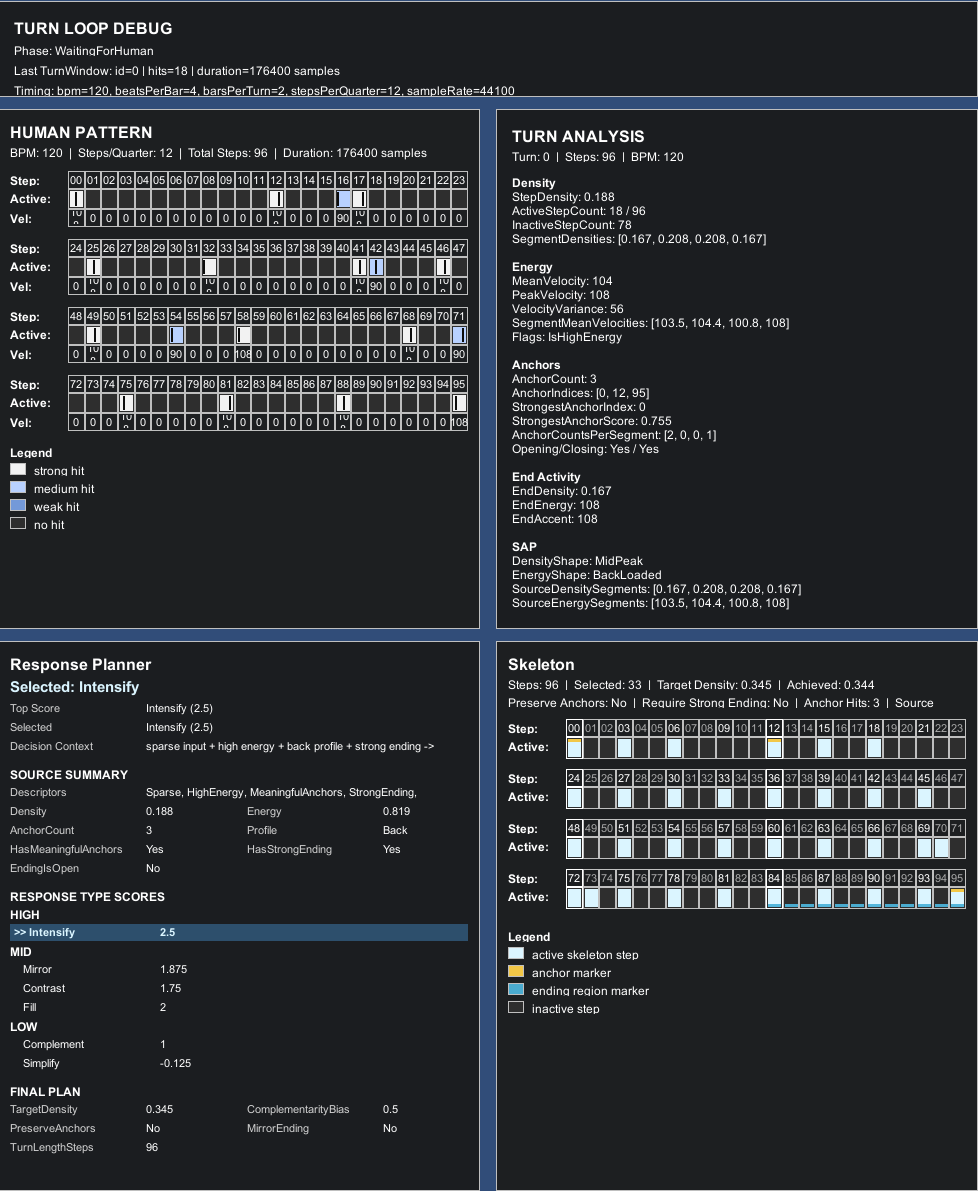
\includegraphics[width=\textwidth]{Figures/4 Figs/Screenshot 2026-04-28 111500.png}
\caption{Integrated runtime debug panel exposing human pattern, analysis, planner and skeleton state.}
\label{fig:debug-panel-runtime}
\end{figure}

\subsection{Runtime I/O Visualisation}\label{runtime-io-visualisation}

Real-time phrase visualisation is achieved through panels with
grid-based representations of PatternTurn objects. Each step is a cell
with intensities denoted by colour and numerical value. This allows
comparison between human and AI responses.

\begin{figure}[htbp]
\centering
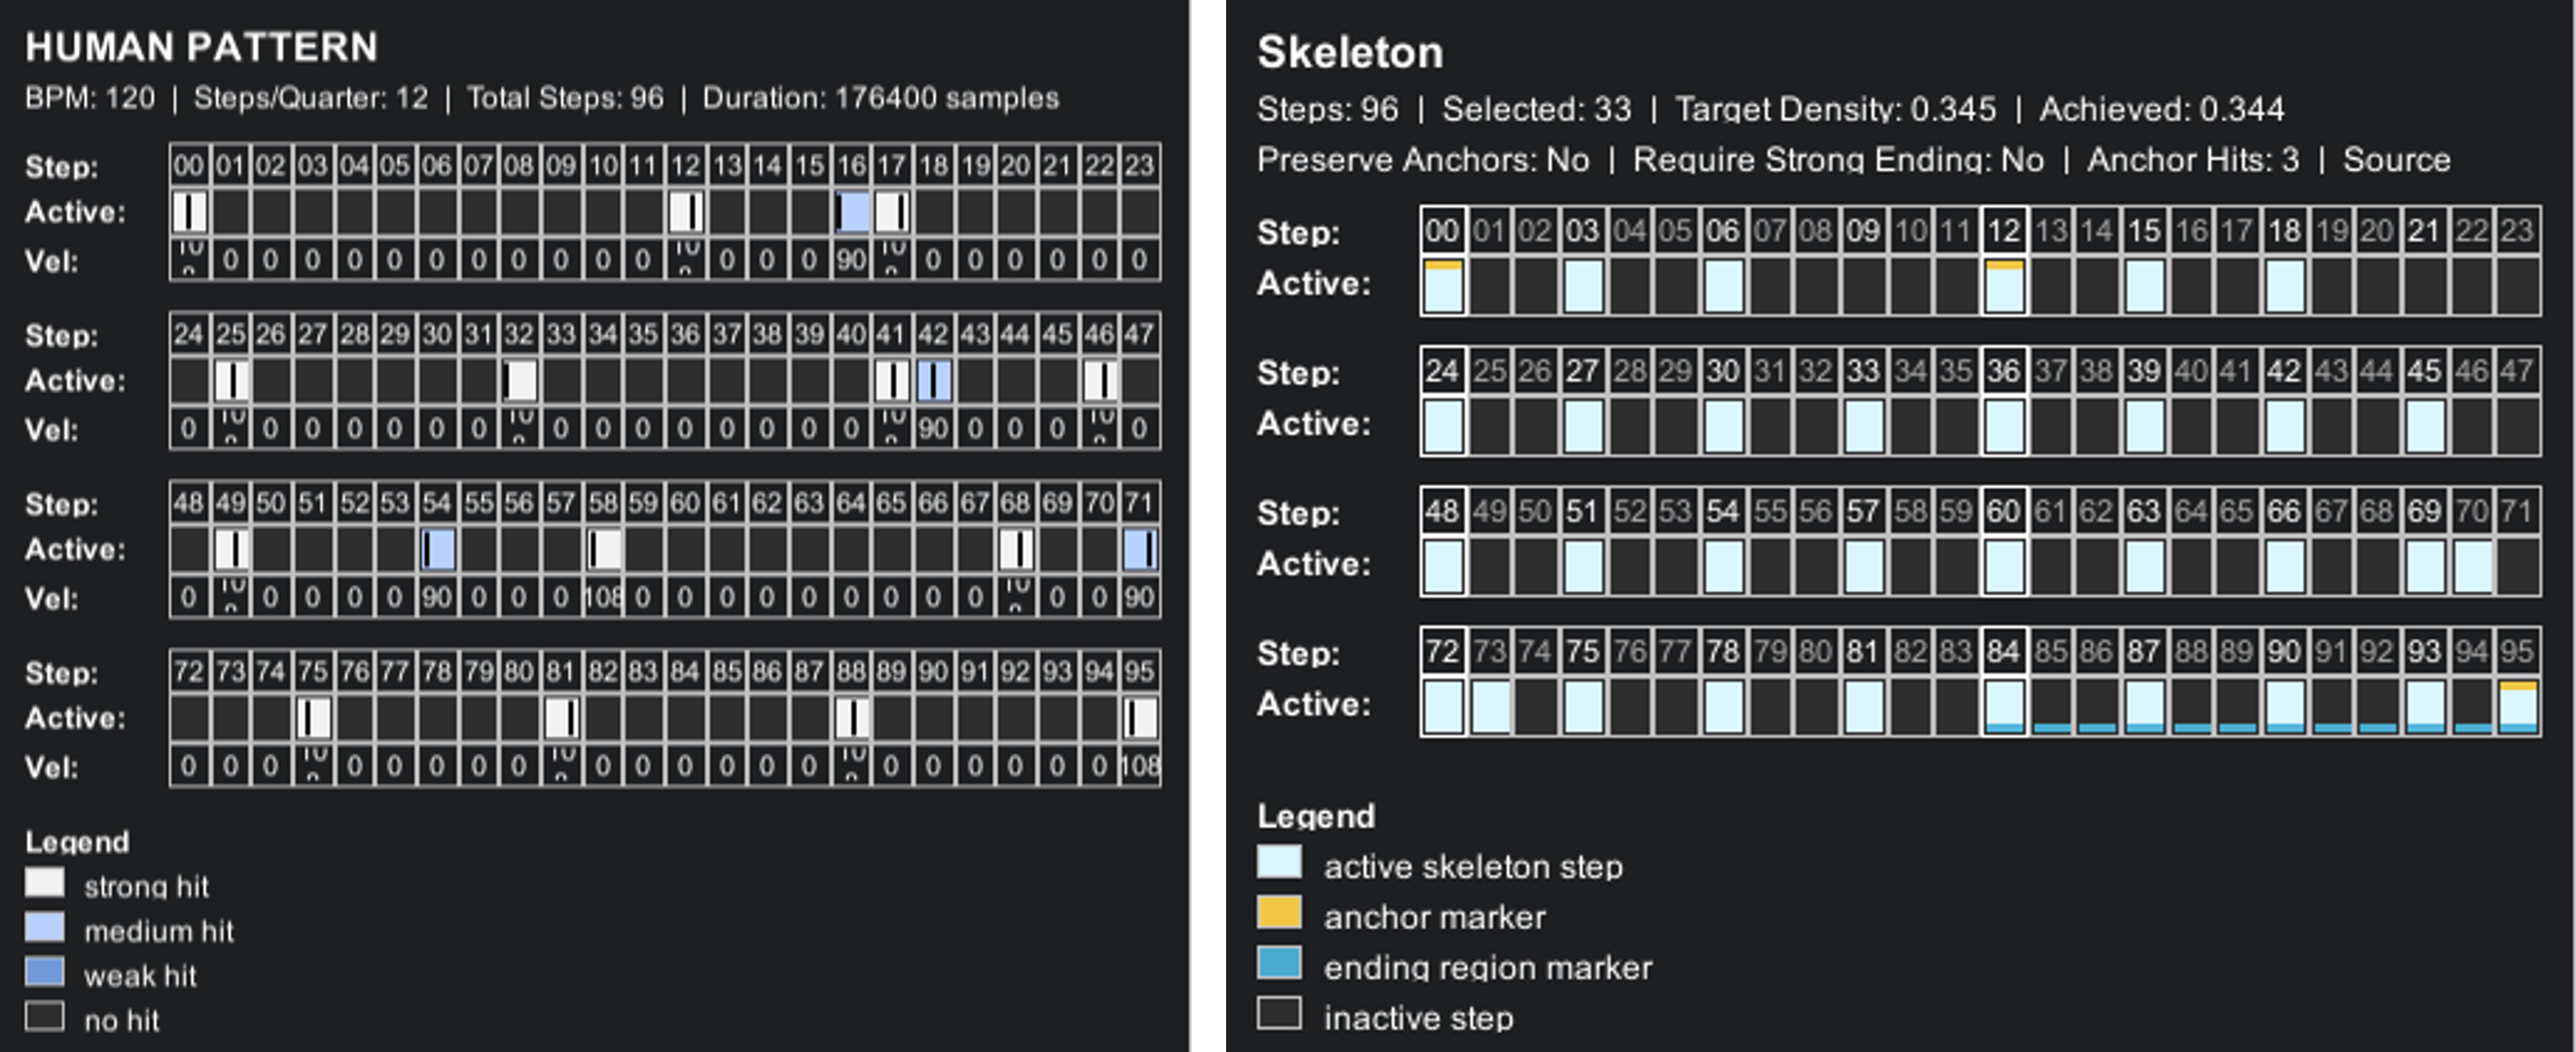
\includegraphics[width=\textwidth]{Figures/4 Figs/Pattern x Skeleton.png}
\caption{Runtime visualisation comparing pattern and skeleton representations.}
\label{fig:pattern-skeleton-runtime}
\end{figure}

\subsection{Analysis Feature Values}\label{analysis-feature-values}

\begin{figure}[htbp]
\centering
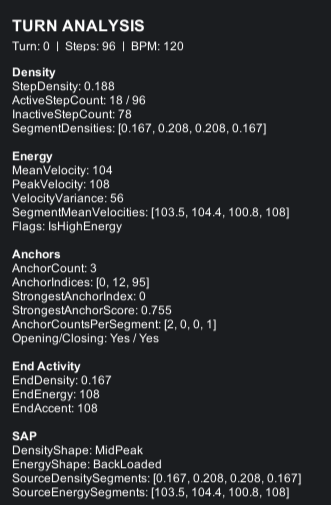
\includegraphics[width=\textwidth]{Figures/4 Figs/Turn Analysis.png}
\caption{TurnAnalysis debug panel showing extracted rhythmic feature values.}
\label{fig:turn-analysis-debug}
\end{figure}

The Turn Analysis Debug panel produces a structured debug snapshot
capturing its internal decision process. This includes the score
breakdowns per feature family including values that indicate
relationships at the bar level. This illuminates the precursor stages to
the Planner.

\subsection{Planner Decision Trace}\label{planner-decision-trace}

\begin{figure}[htbp]
\centering
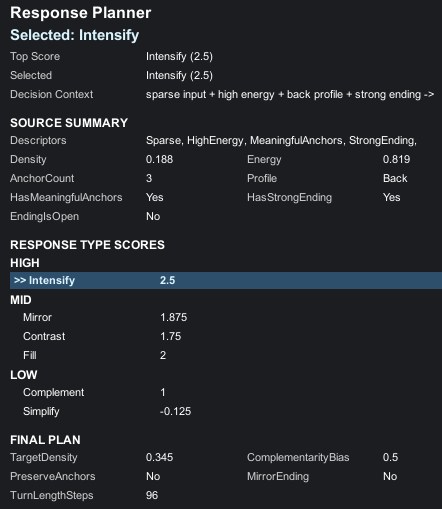
\includegraphics[width=\textwidth]{Figures/4 Figs/Response Planner.png}
\caption{ResponsePlanner debug panel showing scores, descriptors and selected response parameters.}
\label{fig:response-planner-debug}
\end{figure}

The ResponsePlanner also produces a structured debug snapshot capturing
its decision trace. This includes scores, contextual feature
classifications and derived plan parameters. By exposing these values,
the system allows each decision to be traced from analysed features to
final response selection.

\subsection{Structural Generation Visualisation}\label{structural-generation-visualisation}

\begin{figure}[htbp]
\centering
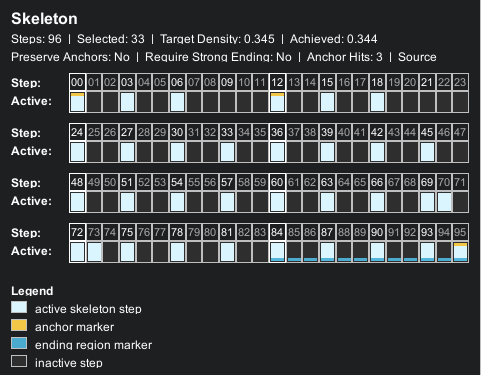
\includegraphics[width=\textwidth]{Figures/4 Figs/Skeleton.png}
\caption{SkeletonBuilder visualisation showing selected structural response steps.}
\label{fig:skeleton-debug}
\end{figure}

The SkeletonBuilder exposes per-step selection results, allowing the
structural generation process to be visualised. This makes it possible
to analyse how factors such as metrical weighting, anchor preservation
and density constraints interact during the selection process.

\subsection{Offline Diagnostics}\label{offline-diagnostics}

\begin{figure}[htbp]
\centering
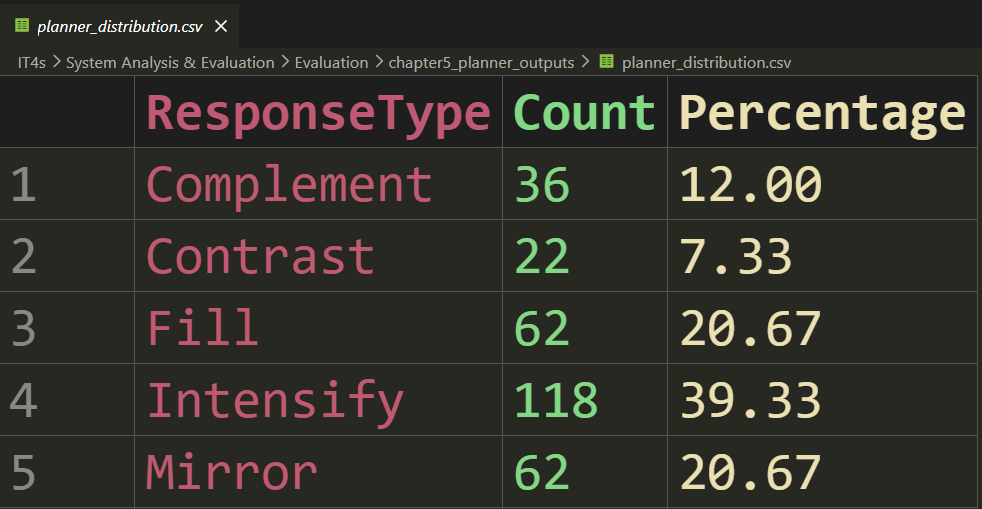
\includegraphics[width=\textwidth]{Figures/4 Figs/planner_distribution.png}
\caption{Offline diagnostic output summarising planner response distributions.}
\label{fig:offline-diagnostics}
\end{figure}

In addition to runtime tools, the system includes offline diagnostic
infrastructure for batch evaluation. SyntheticPatternTurn inputs are
processed through the analysis and planning stages, with outputs
exported as structured data.

Typical recorded data includes:

\begin{itemize}
\item
  response type scores
\item
  selected strategies
\item
  feature distributions
\item
  structural metrics
\end{itemize}

These outputs are stored in formats such as CSV, enabling quantitative
analysis and reproducible experimentation.

\subsection{Data logging and traceability}\label{data-logging-and-traceability}

All major components expose structured outputs:

\begin{itemize}
\item
  TurnAnalysisResult \(\rightarrow\) feature values
\item
  ResponsePlannerDebugSnapshot \(\rightarrow\) decision trace
\item
  SkeletonPattern \(\rightarrow\) structural output
\end{itemize}

This ensures that system behaviour is fully reproducible:

\begin{itemize}
\item
  identical inputs produce identical outputs
\item
  intermediate states can be re-examined
\item
  edge cases can be isolated and analysed
\end{itemize}

\subsection{Role in System Architecture}\label{role-in-system-architecture-5}

The observability layer enables the system to function as an inspectable
computational model, rather than a black-box generator. By exposing
intermediate representations and decision processes, it provides the
foundation for both debugging and formal evaluation.
